% Test case 1. This should succeed.
% Tests of timecode functionality of the preview script.

\mag=1200

%%% VSV IN-VIDEO TEMPLATE
%%% MATTHEW IRELAND, 23 JULY MMXV

\documentclass[10pt]{article}

%%% VSV IN-VIDEO TEMPLATE
%%% MATTHEW IRELAND, 23 JULY MMXV

% PACKAGES USED IN VSV TEMPLATE
% FEEL FREE TO ADD TO THIS LIST

\usepackage[utf8]{inputenc}
\usepackage{amsmath}
\usepackage{amssymb}
\usepackage{graphicx}
\usepackage{fancyhdr}
\usepackage{color,soul}
\usepackage[table,usenames,dvipsnames]{xcolor} % table cell colouring
\usepackage{array,multirow,graphicx}
\usepackage{longtable}     % split large tables over page boundaries
\usepackage{hhline}
\usepackage{enumerate}
\usepackage{hyphenat}
\usepackage{fancyvrb}
\usepackage{epstopdf}
\usepackage{semantic} % for inference rules
\usepackage[utf8]{inputenc}
\usepackage{changepage}   % adjustwidth environment
\usepackage{cleveref} % referencing with § character
\usepackage{framed,color}
\usepackage{makecell}
\usepackage[font=small,labelfont=bf]{caption} % small captions, bold labels
\usepackage{lipsum}
\usepackage{listings}      % source-code listings
\usepackage{todonotes}     % todo notes (inc. placeholder images)
\usepackage{siunitx}       % si units
\usepackage{float} % custom floats and for 'H' placement specifier on figures
\usepackage{complexity}    % complexity classes typesetting
\usepackage{pdftexcmds}    % conditionals (for setting text width)
\usepackage{mdframed}
\usepackage{upquote}% getting the right grave ` (and not ‘)!
\usepackage{hyperref}
\usepackage{bookmark}


% tikz
\usepackage{pgf}
\usepackage{tikz}
\usetikzlibrary{arrows,shapes,trees,backgrounds,automata,patterns}


%%%% PDFINFO FOR PDFTEX %%%%
\pdfinfo{/Author (jkf21 or mti20)
         /Title (VSV)
         /Keywords (vsv)}
%%%% END PDFINFO %%%%


%% Common layout elements
%% Matthew Ireland, 23 July MMXV

% Font definitions
% Upgraded from those in FHK's FORMAT.tex to use
% Latin Modern for vectorization & additional glyphs.
\usepackage{lmodern}
\usepackage[T1]{fontenc}


% Length definitions
\makeatletter
\g@addto@macro\normalsize{%
 %% page layout
   % see corresponding documents for left/right frames
 %% paragraphs
   \setlength{\baselineskip}{12pt plus 0pt minus 0pt}
   \setlength{\parskip}{12pt plus 0pt minus 0pt}
   \setlength{\parindent}{0pt plus 0pt minus 0pt}
 %% floats
   \setlength{\floatsep}{12pt plus 0 pt minus 0pt}
   \setlength{\textfloatsep}{20pt plus 0pt minus 0pt}
   \setlength{\intextsep}{14pt plus 0pt minus 0pt}
   \setlength{\dbltextfloatsep}{20pt plus 0pt minus 0pt}
   \setlength{\dblfloatsep}{14pt plus 0pt minus 0pt}
 %% maths
   \setlength{\abovedisplayskip}{12pt plus 0pt minus 0pt}
   \setlength{\belowdisplayskip}{12pt plus 0pt minus 0pt}
 %% lists
   \setlength{\topsep}{10pt plus 0pt minus 0pt}
   \setlength{\partopsep}{3pt plus 0pt minus 0pt}
   \setlength{\itemsep}{5pt plus 0pt minus 0pt}
   \setlength{\labelsep}{8mm plus 0mm minus 0mm}
   \setlength{\parsep}{\the\parskip}
   \setlength{\listparindent}{\the\parindent}
 %% verbatim
   \setlength{\fboxsep}{5pt plus 0pt minus 0pt}
}
\makeatother


% PERMIT GAPPY TEXT IN PREFERENCE TO HYPHENS
\hyphenpenalty=10000
\tolerance=10000


% make links not-ugly
\hypersetup{
    colorlinks=false,
    pdfborder={0 0 0},
}

%%%% referencing with § character %%%%
\crefformat{section}{§#2#1#3}
\crefname{section}{§}{§§}
\Crefname{section}{§}{§§}

% frames
\definecolor{shadecolor}{rgb}{1,0.8,0.3}


% tables -- centre text vertically
\newcolumntype{L}[1]{>{\raggedright\let\newline\\\arraybackslash\hspace{0pt}}m{#1}}
\newcolumntype{C}[1]{>{\centering\let\newline\\\arraybackslash\hspace{0pt}}m{#1}}
\newcolumntype{R}[1]{>{\raggedleft\let\newline\\\arraybackslash\hspace{0pt}}m{#1}}


%%% VSV macro definitions


% FHK's \marks definition, repackaged as LaTeX
\newcommand{\vsvmarks}[1]{{\unskip \nobreak \hfil \penalty 50 \hskip 8pt
                \hbox{}\nobreak \hfil \setbox0=\hbox{#1}%
                [\ifdim \wd0>11pt #1\else #1 mark\ifnum #1=1\else s\fi\fi]%
                \parfillskip=0pt \finalhyphendemerits=0\par}}

% FHK's \def macro, to be repackaged as LaTeX (TODO)
\def \Def {\buildrel {\rm def} \over = }

% TDJ's \examhead
\newcommand{\vsvexamhead}[3]{\section{#1 Paper #2 Question #3}}

% This is an attempt to implement FHK's \beginquestion in LaTeX
% Usage: \begin{vsvquestion}{<year>}{<paper>}{<question num>}
\newenvironment{vsvoldquestion}[3]%
 {\subsection*{#1 Paper #2}\begin{minipage}[t]{24pt}{\textbf{#3}}\end{minipage}\begin{minipage}{\textwidth-24pt}}
 {\end{minipage}\vspace{12pt}}


% This is a better way to do questions
\newenvironment{vsvquestion}[3]%
 {\subsection*{#1 Paper #2 Question #3}}
 {\vspace{12pt}}


\newcommand{\vsvitem}[3]{\item}

\definecolor{hlcolour}{rgb}{1,1,0}
\sethlcolor{hlcolour}
%\newcommand{\vsvhl}[1]{\hspace{-2pt}\hl{\mbox{}~#1~\mbox{}}\hspace{-2pt}}
\newcommand{\vsvhl}[3]{\hl{#3}}

\newcommand{\vsvhlnowrap}[3]{\colorbox{hlcolour}{{#3}}}

\setstcolor{red}
\newcommand{\vsvcorrect}[4]{\st{#3}\ \ \ \ \ #4}
\newcommand{\vsvxcorrect}[2]{\vsvcorrect{}{}{#1}{#2}}
\newcommand{\vsvxxcorrect}[2]{#1}

\lstdefinestyle{customc}{
  belowcaptionskip=1\baselineskip,
  breaklines=true,
  xleftmargin=\parindent,
  language=C,
  showstringspaces=false,
  basicstyle=\fontsize{11pt}{13pt}\selectfont\ttfamily,
  columns=flexible,
  keepspaces=true,
  keywordstyle=\bfseries\color{green!40!black},
  commentstyle=\itshape\color{purple!40!black},
  identifierstyle=\color{blue},
  stringstyle=\color{orange},
  escapechar=~
}




\newenvironment{vsvgrey}[2]{\leavevmode\color{gray}}{\leavevmode\color{black}}

\newenvironment{vsvappear}[2]{}{}

\newcommand{\nosection}[1]{%
  \refstepcounter{section}%
  \addcontentsline{toc}{section}{\protect\numberline{\thesection}#1}%
  \markright{#1}}


%%%% preview environment %%%%
\newcounter{vsvrhscounter}
\newcounter{vsvlhscounter}
\makeatletter
\newcommand\vsvsetwidth[3]{%
  \ifnum\pdf@strcmp{\unexpanded{#1}}{right}=0 %
     \expandafter\@firstoftwo
  \else
    \expandafter\@secondoftwo
  \fi
    {\eject \pdfpageheight=171mm \newgeometry{textheight=143mm,textwidth=129mm,top=28mm,bottom=10mm,left=14mm,showframe=true}\fancyhf[LC]{}\fancyhf[HC]{\textbf{Question (right-hand) pane -- Number R\thevsvrhscounter}\\In: #2 --- Out: #3}\stepcounter{vsvrhscounter}}
    {\eject \pdfpageheight=105mm \newgeometry{textheight=67mm,paperwidth=149mm,textwidth=129mm,top=28mm,bottom=10mm,left=14mm,showframe=true}\fancyhf[LC]{}\fancyhf[HC]{\textbf{Image/code (left-hand) pane -- Number L\thevsvlhscounter}\\In: #2 --- Out: #3}\stepcounter{vsvlhscounter}}%
}
\makeatother



\newenvironment{vsvframe}[3]{%
\vsvsetwidth{#3}{#1}{#2}
\thispagestyle{fancy}

\begin{mdframed}
}%
{\end{mdframed}

\eject \pdfpageheight=297mm
\restoregeometry
\pagestyle{empty}}


\usepackage{geometry}
\usepackage{a4}

\begin{document}
\raggedbottom


\begin{vsvframe}{1-0:00.000}{1-5:00}{right}
\vsvhl{1-0:10}{1-0:20}{This frame is designed to test the ungreying of an environment, and then a bulleted list.}

\begin{vsvgrey}{}{1-0:30}
\lipsum[66]
\end{vsvgrey}

\begin{itemize}
\vsvitem{}{1-0:40}{grey}
\lipsum[68]
\vsvitem{}{1-0:50}{grey}
\lipsum[75]
\vsvitem{}{1-1:00}{grey}
Here's a bullet point worth 12 marks.\vsvmarks{12}
\vsvitem{}{1-1:10}{grey}
And here's a longer one so that marks should move on to the next line.\vsvmarks{10}
\end{itemize}

\begin{vsvgrey}{}{1-1:20}
And then finally this environment will ungrey until the end of the frame.
\end{vsvgrey}

\end{vsvframe}

\begin{vsvframe}{1-0:00}{1-5:00.10}{left}
\vsvhl{1-0:9.50}{1-00:020.60}{This frame is designed to test code correction.}

\lstset{columns=flexible,style=customc}
\begin{lstlisting}
~ \vsvcorrect{1-0:30}{}{tmp1=a*b}{tmp1=a-b} ~
 x = tmp1+c;    // this is a comment
\end{lstlisting}

\begin{vsvappear}{1-0:40}{}
And so you can see text was corrected!
\end{vsvappear}

\end{vsvframe}


\begin{vsvframe}{1-5:00}{1-10:00.01}{right}
\vsvhl{1-5:10}{1-5:20}{This frame is designed to test appearance of items in a list and image includes.}

\begin{vsvappear}{1-5:30}{}
This text will appear! Hello cruel world, from this paragraph!
\end{vsvappear}

\begin{enumerate}
\vsvitem{1-5:40}{}{appear}
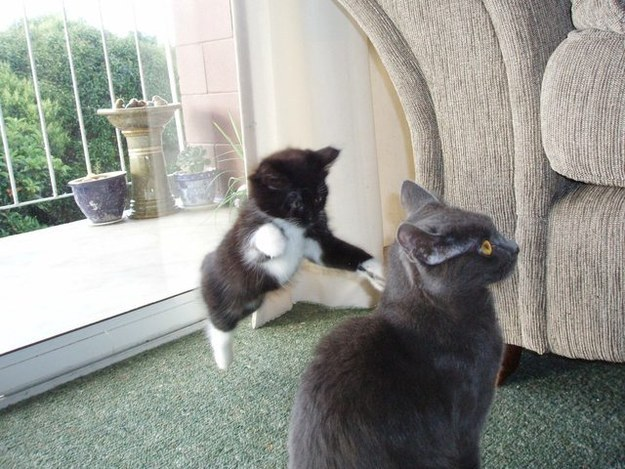
\includegraphics[scale=0.2]{img/0001.jpg}

\vsvitem{1-5:50}{}{appear}

\includegraphics[scale=0.2]{img/0002.jpg}

\vsvitem{1-06:00}{}{appear}
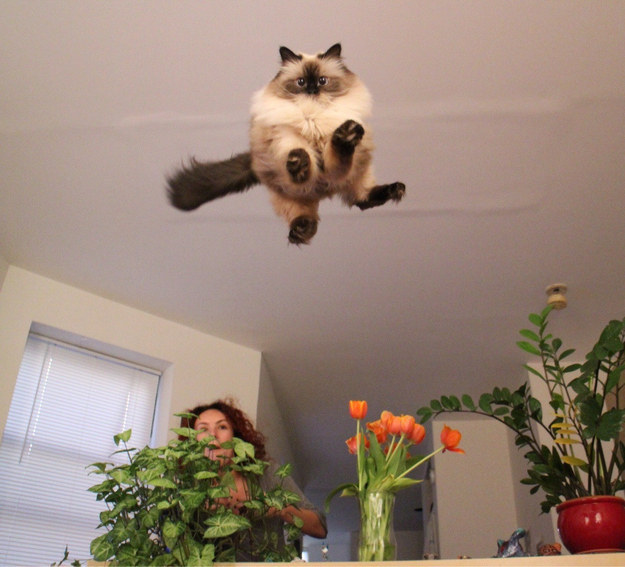
\includegraphics[scale=0.2]{img/0003.jpg}
\end{enumerate}
\end{vsvframe}

\begin{vsvframe}{1-5:00}{1-10:00.01}{left}
More image includes...

\begin{enumerate}
\vsvitem{1-6:000000000000000010}{}{appear}

\includegraphics[scale=0.1]{img/0004.jpg}
\end{enumerate}

\begin{vsvappear}{1-00000000000000006:20}{}
And one final piece of text to appear!


\includegraphics[scale=0.1]{img/0005.jpg}
\end{vsvappear}

\end{vsvframe}

\begin{vsvframe}{1-10:00.01}{2-5:00}{left}
\vsvhl{}{}{This is a cross-segment frame.}


% TODO do a strikethrough in a bullet point
% TODO description list

\end{vsvframe}

\end{document}

